\documentclass[a4paper,12pt,halfparskip,DIV14]{scrartcl}

\newcommand{\dokumenttitel}{Analyse}
\usepackage{../bodesuri}
\usepackage{multicol}


\begin{document}

\title{\dokumenttitel}
\titlehead{
	\centering
	
\includegraphics[width=0.5 \textwidth, clip, trim = 0 7cm 0 0]{design/externes_design/bodesuri_plakat}
	\vspace{2cm}
}
\author{Danilo~Couto, Philippe~Eberli, \\ Pascal~Hobus, Reto~Schüttel, Robin~Stocker}
\maketitle
\newpage

\pagenumbering{roman}

\tableofcontents
\thispagestyle{plain}
\newpage

\pagenumbering{arabic}

\markright{Bodesuri -- \dokumenttitel}


\section{Use Cases und Funktionale Anforderungen} 
\subsection{Use Case Diagramm}\label{sub:use_case_diagramm} 
\begin{figure}
	[htp] \centering 
	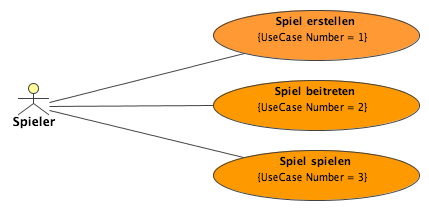
\includegraphics[width=0.8\textwidth]{UseCaseDiagramm.png} \caption{Use Case Diagramm}\label{fig:UseCaseDiagramm.png} 
\end{figure}

\subsection{Aktoren}\label{sec:aktoren} 
\begin{itemize}
	\item \textbf{Spieler}: Spielt das Spiel. 
\end{itemize}

\subsection{Personas}\label{sec:personas} 

\subsubsection{Hans Müller}\label{sub:hans_müller} 

Hans Müller, 28, Familienvater. Er ist gelernter Kaufmann und arbeitet als Sachbearbeiter bei einer Bank. Er nutzt den PC regelmäsig im Geschäft (Office, SAP und bankeigene Software). Surft privat ab und zu mal im Netz, um dort Informationen einzuholen. Kennt sich aber sonst eher wenig mit PCs aus. 

Er spielt seit mehreren Jahren angefressen Dog. Zu Spitzenzeiten bis zu 3 Mal pro Woche. Er möchte Bodesuri nutzen, damit er einfacher auf die Schnelle mit seinen Kollegen zocken kann. 

\subsubsection{Maria Lehner}\label{sub:maria_lehner} 

Maria Lehner, 18, Gymnasiastin. Ist mit dem PC aufgewachsen und hat einen eigenen in ihrem Zimmer stehen. Sie nutzt ihn vor allem um mit ihren Kollegen per MSN zu Chatten und im Internet zu surfen. Ab und zu schreibt sie auch eine Arbeit für die Schule mit Word. Maria möchte später studieren gehen, am liebsten etwas im Bereich Umwelt/Natur, da sie sich dafür interessiert. 

Dog kennt sie von einem Klassenkollegen, der sie letzte Woche zu sich nach Hause zu einem Turnier eingeladen hat. Sie hat verloren und möchte nun etwas üben.

\subsection{Beschreibung der Use Cases}\label{sub:use_cases}
\subsubsection{UC01: Spiel erstellen}\label{ssub:uc01_spiel_erstellen}
Der Benutzer der das Spiel beherbergt startet die Serverapplikation.

\begin{tabular}{@{} l l @{}}
	\textbf{Aktor:}											&	Spieler \\
	\textbf{Vorbedingungen:}						& Keine \\
	\textbf{Nachbedingungen:}						& Keine \\
	\textbf{Häufigkeit des Auftretens:}	& Einmal pro Spiel \\
\end{tabular}

\vspace{0.5cm}

\begin{multicols}{2}
\raggedcolumns
\paragraph{Actor Action}
\begin{enumerate}
	\item[1] Spieler startet den Server
\end{enumerate}
\columnbreak
\paragraph{System Response}
\begin{enumerate}
	\item[2] System startet den Server
	\item[3] System bestätigt korrektes Funktionieren des Servers
\end{enumerate}
\end{multicols}
\paragraph{Alternative Abläufe}
\begin{enumerate}
	\item[2a] Start des Servers schlägt fehl.
	\begin{enumerate}
		\item System benachrichtigt den Benutzer.
		\item Benutzer behebt den Fehler.
		\item Use Case wird wiederholt.
	\end{enumerate}
\end{enumerate}

\subsubsection{UC02: Spiel beitreten}\label{ssub:uc02_spiel_beitreten}
Der Spieler gibt einen Server an, zu welchem das System eine Netzverbindung erstellt. Sobald vier Spieler dem Spiel beigetreten sind wird das Spiel begonnen.

\begin{tabular}{@{} l l @{}}
	\textbf{Aktor:}											&	Spieler \\
	\textbf{Vorbedingungen:}						& Ein laufender Server \\
	\textbf{Nachbedingungen:}						& Spieler beigetreten \\
	\textbf{Häufigkeit des Auftretens:}	& Einmal pro Spiel und Spieler \\
\end{tabular}

\vspace{0.5cm}

\begin{multicols}{2}
\raggedcolumns
\paragraph{Actor Action}
\begin{enumerate}
	\item[1] Spieler gibt Verbindungsdaten zu einem bestimmten Server ein.
\end{enumerate}
\columnbreak
\paragraph{System Response}
\begin{enumerate}
	\item[2] System verbindet sich mit dem Server
	\item[3] System bestätigt erfolgreiche Verbindung und wartet bis der Server meldet, dass das Spiel vollständig ist.
	\item[4] System erhält vom Server die Meldung, dass das Spiel beginnt.
\end{enumerate}
\end{multicols}
\paragraph{Alternative Abläufe}
\begin{enumerate}
	\item[*a] Benutzer bricht Verbindung ab.\newline
	Das System benachrichtigt den Server.
	\item[2a] Verbindung zum Server schlägt fehl.
	\begin{enumerate}
		\item System benachrichtigt den Benutzer.
		\item Benutzer überprüft seine Einstellungen.
		\item Use Case wird wiederholt.
	\end{enumerate}
	\item[2b] Das Spiel hat bereits begonnen.\newline
	Der Benutzer sucht einen anderen oder startet seinen eigenen Server.
\end{enumerate}

\subsubsection{UC03: Spiel spielen}\label{ssub:uc03_spiel_erstellen}
Das System verteilt allen Spielern Spielkarten. Jeder Spieler tauscht mit seinem Partner eine Karte. Danach werden reihum je eine Karte gezogen und die Spielfiguren entsprechend bewegt. Wenn die Spieler alle ihre Karten gespielt haben, verteilt das System wieder neue Karten und eine neue Runde beginnt. 

\begin{tabular}{@{} l l @{}}
	\textbf{Aktor:}														&	Spieler \\
	\textbf{Vorbedingungen:}									& Ein Server mit vier angemeldeten Spielern \\
	\textbf{Nachbedingungen:}									& Der Server ist korrekt beendet \\
	\textbf{Häufigkeit des Auftretens:}				& Von einmal pro Woche bis 2--3 Mal pro Jahr \\
\end{tabular}
\newpage
\begin{multicols}{2}
\raggedcolumns
\paragraph{Actor Action}
\begin{enumerate}
	\item[]
	\item[]
	\item[3] Spieler wählt Karte aus die er mit dem Partner tauschen will
	\item[]
	\item[]
	\item[7] Spieler wählt Karte die er spielen will aus und erfasst den Zug den er damit machen will.
\end{enumerate}
\emph{Schritte 6-10 werden wiederholt bis kein Spieler mehr Karten hat.\newline
Schritte 2-10 werden wiederholt bis eine Gruppe gewonnen hat.}
\columnbreak
\paragraph{System Response}
\begin{enumerate}
	\item[1] System initialisiert Spielbrett
	\item[2] System erhält Spielkarten vom Server
	\item[4] System übermittelt getauschte Karte an den Server.
	\item[5] System erhält getauschte Karte vom Server.
	\item[6] System wartet bis der Benutzer am Zug ist und visualisiert die Züge der anderen Benutzer.
	\item[8] System validiert den Zug und übermittelt ihn an der Server.
	\item[9] Server bestätigt den Zug.
	\item[10] System visualisiert den Zug.
\end{enumerate}
\end{multicols}
\paragraph{Alternative Abläufe}
\begin{enumerate}
	\item[*a] Benutzer verlässt das Spiel.
	\begin{enumerate}
		\item System benachrichtigt den Server, welcher alle anderen Spieler benachrichtigt.
		\item Spiel wird beendet.
	\end{enumerate}
	\item[*b] Server nicht mehr erreichbar.
	\begin{enumerate}
		\item System benachrichtigt den Benutzer.
		\item Spiel wird beendet.
	\end{enumerate}	\item[7a] Benutzer kann keine Karte spielen.\newline
	Das System benachrichtigt den Server, dass der Spieler diese Runde nicht mehr spielen kann.
	\item[8a] Der angeforderte Zug ist ungültig.
	\begin{enumerate}
		\item System benachrichtigt den Benutzer.
		\item Benutzer macht einen anderen Zug.
		\item Validierung wird wiederholt.
	\end{enumerate}
	\item[10a] Der Spieler hat gewonnen.
	\begin{enumerate}
		\item Der Partner hat auch schon gewonnen.\newline
		Das System zeigt an welche Gruppe gewonnen hat und zeigt eine kleine Rangliste.
		\item Der Partner hat noch nicht gewonnen.
		\begin{enumerate}
			\item System benachrichtigt den Server.
			\item System schaltet die Figuren des Partners frei.
		\end{enumerate}
	\end{enumerate}
\end{enumerate}

\section{Nichtfunktionale Anforderungen}\label{cha:nichtfunktionale_anforderungen} % (fold)

\subsection{Leistungs- und Mengenanforderungen}\label{sub:leistungs_und_mengenanforderungen} % (fold)
\subsubsection{Leistungsanforderungen}\label{ssub:leistungsanforderungen} % (fold)
\begin{itemize}
	\item Damit der Spielfluss nicht gestört wird, soll ein Spielzug in maximal drei Sekunden über das Netzwerk synchronisiert sein.
	\item Der Spielstand muss nach jedem Zug bei allen Spielern konsistent sein. Inkonsistenzen bzw. Synchronisationsprobleme sollten sofort zu einem kontrollierten Spielabbruch führen.\footnote{Das Client/Server-Modell sieht nur in zwei Fällen solche Fehler vor: Bei Verbindungsproblemen und bei Fehlern in der Applikation selber. In beiden Situationen ist eine automatische Fehlerkorrektur nicht vorgesehen.}
\end{itemize}
% subsubsection leistungsanforderungen (end)
\subsubsection{Mengenanforderungen}\label{ssub:mengenanforderungen} % (fold)
\begin{itemize}
	\item Ein Server beherbergt immer nur ein Spiel.
	\item Es müssen genau vier Spieler für ein Spiel vorhanden sein.
	\item Es werden zwei Gruppen à zwei Spieler gebildet.
	\item Der Kartenstapel besteht aus zwei Decks à 52 Karten.
\end{itemize}
% subsubsection mengenanforderungen (end)

\subsubsection{Anforderungen an Schnittstellen}\label{ssub:anforderungen_an_schnittstellen} % (fold)
\paragraph{Benutzerschnittstelle}\label{ssub:benutzerschnittstelle} % (fold)
\begin{itemize}
	\item Das GUI soll so weit wie möglich nur mit der Maus bedienbar sein.
	\item (FIXME: ist das hier und so wirklich sinnvoll?) Das GUI repräsentiert jeweils ein Dog-Spielbrett mit den daraufliegenden Figuren.
	\item (FIXME: ist das hier und so wirklich sinnvoll?) Die Karten und der Kartenstapel werden im GUI visuell dargestellt.
\end{itemize}
% paragraph benutzerschnittstelle (end)
\paragraph{Hardware-Schnittstelle}\label{ssub:hardware_schnittstelle} % (fold)
Das Spiel wird in Java entwickelt und ist plattformunabhängig. Es wird keine weitere Hardware benötigt.
% paragraph hardware_schnittstelle (end)
\paragraph{Software-Schnittstelle}\label{ssub:software_schnittstelle} % (fold)
\begin{itemize}
	\item Java 5
	\item Swing
	\item Java 2D
	\item Java RMI
\end{itemize}
% paragraph software_schnittstelle (end)
\paragraph{Datenhaltung}\label{ssub:datenhaltung} % (fold)
Es wird keine persistente Datenhaltung benötigt. Alle Daten werden jeweils nur in einer Session benötigt und müssen deshalb nicht permanent gespeichert werden.
% paragraph datenhaltung (end)
\paragraph{Kommunikationsschnittstelle}\label{ssub:kommunikationsschnittstelle} % (fold)
\begin{itemize}
	\item Als Kommunikations-Framework wird RMI verwendet.
	\item Für ein Spiel ist ein Server unabdingbar.
	\item Jeder teilnehmende Spieler stellt einen Client dar.
\end{itemize}
% paragraph kommunikationsschnittstelle (end)
% subsubsection anforderungen_an_schnittstellen (end)

\subsection{Anforderungen im Einzelnen}\label{sub:anforderungen_im_einzelnen} % (fold)
\subsubsection{Randbedingungen für den Entwurf}\label{ssub:randbedingungen_für_den_entwurf} % (fold)

Als Code-Richtlinien werden weitgehend die "<Sun Coding Guidelines"> übernommen (siehe separates Dokument).

\paragraph{Einschränkungen bezüglich Software}\label{ssub:einschränkungen_bzgl_software} % (fold)
\begin{itemize}
	\item Java 5
	\item Betriebssysteme
	\begin{itemize}
		\item Mac OS X
		\item Windows XP
		\item GNU/Linux
	\end{itemize}
\end{itemize}

% paragraph einschränkungen_bzgl_software (end)

\paragraph{Einschränkungen bezüglich Hardware}\label{ssub:einschränkungen_bzgl_hardware} % (fold)

Für die Verwendung des Spiels ist ein netzwerkfähiger Computer vorausgesetzt.

% paragraph einschränkungen_bzgl_hardware (end)
% subsubsection randbedingungen_für_den_entwurf (end)
% subsection anforderungen_im_einzelnen (end)

\subsubsection{Merkmale}\label{ssub:merkmale} % (fold)
\paragraph{Sicherheit}\label{ssub:sicherheit} % (fold)
\begin{itemize}
	\item Kommunikation zwischen Client und Server ist nicht verschlüsselt.
	\item Die Einhaltung der Spielregeln und der Datenkonsistenz wird sowohl im Client als auch im Server für jede Aktion geprüft.
	\item WEG Das Spiel macht sich implizit die eingebauten Sicherheitsmechanismen von Java (Typsicherheit) und RMI (bewährte Netzwerkkommunikation) zu Nutzen.
\end{itemize}
% paragraph sicherheit (end)

\paragraph{Wartbarkeit}\label{ssub:wartbarkeit} % (fold)

\begin{itemize}
	\item FRAGE(haben wir chat nicht bereits drin?) Ein Chat-System soll mit ungefähr drei Personentagen Aufwand integrierbar sein.
	\item Erweiterbarkeit für die Integration in einen Master-Server der im Internet eine Plattform bietet, um einfach einem Spiel beizutreten.
\end{itemize}
% paragraph wartbarkeit (end)
% subsubsection merkmale (end)

\subsubsection{Andere Anforderungen}\label{ssub:andere_anforderungen} % (fold)
\paragraph{Inbetriebnahme/Installation}\label{ssub:inbetriebnahme_installation} % (fold)
\begin{itemize}
	\item Es ist keine Installation oder Konfiguration notwendig.
	\item Die grafische Oberfläche sollte intuitive bedient werden können. (FIXME, sollten wir da kein 'sollte' schreiben). 
\end{itemize}
% paragraph inbetriebnahme_installation (end)
\paragraph{Konfigurierbarkeit}\label{ssub:konfigurierbarkeit} % (fold)
\begin{itemize}
	\item Ausser der Angabe des Spielernamens und des Servers müssen keine Konfigurationen gemacht werden. (FIXME: wollen wir die folgenden beiden Anforderungen nicht durch diesen ersetzen?)
	\item WEG Am Anfang eines Spiels soll ein Spieler seinen Namen/Spitznamen angeben können.
	\item WEG Um einem Spiel beitreten zu können soll ein Spieler lediglich die IP-Adresse oder den Hostnamen des Servers angeben müssen.
\end{itemize}
% paragraph konfigurierbarkeit (end)
% subsubsection andere_anforderungen (end)

\newpage

\section{Domainmodell}\label{cha:domainmodell} % (fold)

\begin{figure}
	[htp] \centering 
	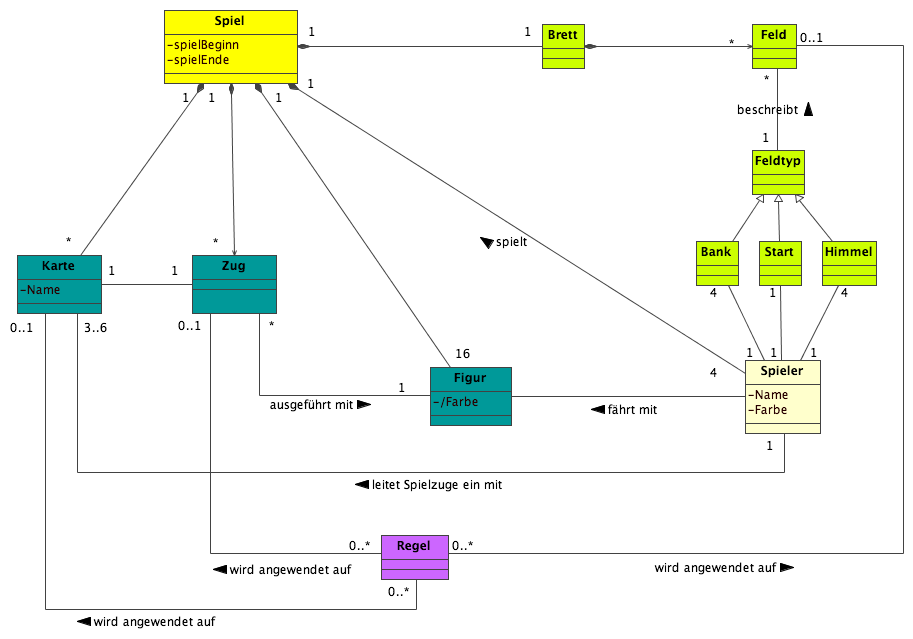
\includegraphics[width=1\textwidth]{DomainModel.png} \caption{Domainmodell}\label{fig:DomainModel.png} 
\end{figure}
\paragraph{Regel}\label{ssub:regel} % (fold)
Eine Regel ist abstrakt. Konkrete Regeln gehören zu einer Karte und werden bei einem Zug überprüft und angewendet. Dieses Regelsystem wird im Design verfeinert.
% paragraph regel (end)
\paragraph{Feldtypen}\label{ssub:feldtypen} % (fold)
Jedem Spieler sind jeweils seine eigenen Instanzen der speziellen Feldtypen Bank, Start und Himmel zugewiesen.
% paragraph feldtypen (end)
% subsection klassenspezifikationen (end)
% chapter domainmodell (end)

\newpage

\section{Systemsequenzdiagramme}\label{cha:systemsequenzdiagramme} % (fold)
\begin{figure}
	[htp] \centering 
	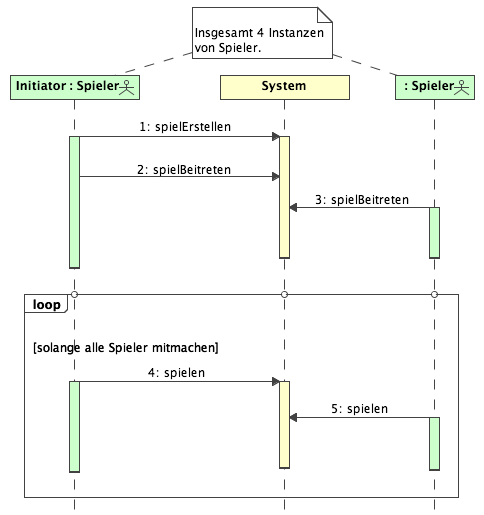
\includegraphics[width=0.8\textwidth]{SystemSequenzDiagramm.png} \caption{Systemsequenzdiagramm des Spiels}\label{fig:SystemSequenzDiagramm.png} 
\end{figure}
% chapter systemsequenzdiagramme (end)
\end{document}
